\documentclass[12pt]{article}
\usepackage{tikz}
\usepackage{amsmath}
% Underlining package
\usepackage{ulem}
\usetikzlibrary{calc}
\usetikzlibrary{angles,quotes}
\usepackage[a4paper, portrait, margin=1cm]{geometry}
\usepackage{fancyhdr}

\newcommand{\HeadingAnswers}{%
\section*{\Large Name: \underline{\hspace{8cm}} \hfill Date: \underline{\hspace{3cm}}}%
\vspace{-3mm}\par
\textbf{Area Rectangles: Answers}\vspace{1pt}\hrule
}

% raise footer with page number; no header
\fancypagestyle{myfancypagestyle}{
  \fancyhf{}% clear all header and footer fields
  \renewcommand{\headrulewidth}{0pt} % no rule under header
  \fancyfoot[C] {\thepage} \setlength{\footskip}{14.5pt} % raise page number allowed min 14.5pt
}
\pagestyle{myfancypagestyle}  % apply myfancypagestyle

\newcounter{minipagecount}

\begin{document}
\HeadingAnswers
\vspace{8mm}

\begin{minipage}{0.55\textwidth}
  \refstepcounter{minipagecount}
  \noindent{(\theminipagecount)}\quad
 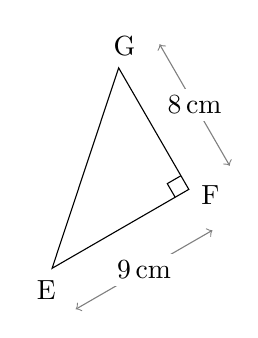
\begin{tikzpicture}[scale=1.0, baseline=(current bounding box.north)]
    \begin{scope}[rotate=30]
        % Draw

        \draw (0,0) coordinate (E) --
         ++(2.005,0) coordinate (F) --
         ++(90:1.782) coordinate (G) -- cycle;

        \pic [draw, -, angle radius=0.2cm] {right angle=G--F--E};

        % Vertex LABELS
        % Labels relative to shape geometry
        \node at ($(E)+(-0.2,-0.2)$) {E};
        \node at ($(F)+(0.2,-0.2)$) {F};
        \node at ($(G)+(0.2,0.2)$) {G};


        % dotted/dashed arrows shifted away from edges
        % Horizontal side (A-B), shifted down
        \draw[<->, gray]
            ($(E) + (0,-0.6cm)$) -- ($(F) + (0,-0.6cm)$)
            node[black, midway, fill=white, inner sep=2.5pt] {9\,cm};

        % Vertical side (B-C), shifted right
        \draw[<->, gray]
            ($(F) + (0.6cm,0)$) -- ($(G) + (0.6cm,0)$)
            node[black, midway, fill=white, xshift=0mm, inner sep=2.5pt] {8\,cm};

    \end{scope}
\end{tikzpicture}
\end{minipage}%
\hfill
\begin{minipage}{.4\textwidth}
  \begin{align*}
    \text{Area} &= \frac{1}{2} \text{bh} \\
    \text{Area} &= \frac{1}{2} \times 9 \text{cm} \times 8 \text{cm}  \\
    \text{Area} &= 36.0 \text{cm}^2
  \end{align*}
\end{minipage}

\par\vspace{1cm}\begin{minipage}{0.55\textwidth}
  \refstepcounter{minipagecount}
  \noindent{(\theminipagecount)}\quad
 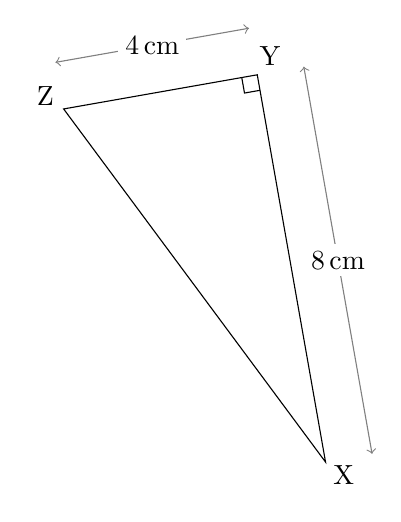
\begin{tikzpicture}[scale=1.0, baseline=(current bounding box.north)]
    \begin{scope}[rotate=100]
        % Draw

        \draw (0,0) coordinate (X) --
         ++(4.994,0) coordinate (Y) --
         ++(90:2.497) coordinate (Z) -- cycle;

        \pic [draw, -, angle radius=0.2cm] {right angle=Z--Y--X};

        % Vertex LABELS
        % Labels relative to shape geometry
        \node at ($(X)+(-0.2,-0.2)$) {X};
        \node at ($(Y)+(0.2,-0.2)$) {Y};
        \node at ($(Z)+(0.2,0.2)$) {Z};


        % dotted/dashed arrows shifted away from edges
        % Horizontal side (A-B), shifted down
        \draw[<->, gray]
            ($(X) + (0,-0.6cm)$) -- ($(Y) + (0,-0.6cm)$)
            node[black, midway, fill=white, inner sep=2.5pt] {8\,cm};

        % Vertical side (B-C), shifted right
        \draw[<->, gray]
            ($(Y) + (0.6cm,0)$) -- ($(Z) + (0.6cm,0)$)
            node[black, midway, fill=white, xshift=0mm, inner sep=2.5pt] {4\,cm};

    \end{scope}
\end{tikzpicture}
\end{minipage}%
\hfill
\begin{minipage}{.4\textwidth}
  \begin{align*}
    \text{Area} &= \frac{1}{2} \text{bh} \\
    \text{Area} &= \frac{1}{2} \times 8 \text{cm} \times 4 \text{cm}  \\
    \text{Area} &= 16.0 \text{cm}^2
  \end{align*}
\end{minipage}

\par\vspace{1cm}\begin{minipage}{0.55\textwidth}
  \refstepcounter{minipagecount}
  \noindent{(\theminipagecount)}\quad
 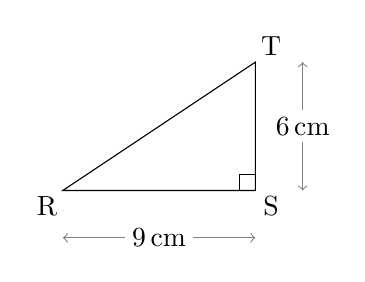
\begin{tikzpicture}[scale=1.0, baseline=(current bounding box.north)]
    \begin{scope}[rotate=0]
        % Draw

        \draw (0,0) coordinate (R) --
         ++(2.446,0) coordinate (S) --
         ++(90:1.631) coordinate (T) -- cycle;

        \pic [draw, -, angle radius=0.2cm] {right angle=T--S--R};

        % Vertex LABELS
        % Labels relative to shape geometry
        \node at ($(R)+(-0.2,-0.2)$) {R};
        \node at ($(S)+(0.2,-0.2)$) {S};
        \node at ($(T)+(0.2,0.2)$) {T};


        % dotted/dashed arrows shifted away from edges
        % Horizontal side (A-B), shifted down
        \draw[<->, gray]
            ($(R) + (0,-0.6cm)$) -- ($(S) + (0,-0.6cm)$)
            node[black, midway, fill=white, inner sep=2.5pt] {9\,cm};

        % Vertical side (B-C), shifted right
        \draw[<->, gray]
            ($(S) + (0.6cm,0)$) -- ($(T) + (0.6cm,0)$)
            node[black, midway, fill=white, xshift=0mm, inner sep=2.5pt] {6\,cm};

    \end{scope}
\end{tikzpicture}
\end{minipage}%
\hfill
\begin{minipage}{.4\textwidth}
  \begin{align*}
    \text{Area} &= \frac{1}{2} \text{bh} \\
    \text{Area} &= \frac{1}{2} \times 9 \text{cm} \times 6 \text{cm}  \\
    \text{Area} &= 27.0 \text{cm}^2
  \end{align*}
\end{minipage}

\par\vspace{1cm}\begin{minipage}{0.55\textwidth}
  \refstepcounter{minipagecount}
  \noindent{(\theminipagecount)}\quad
 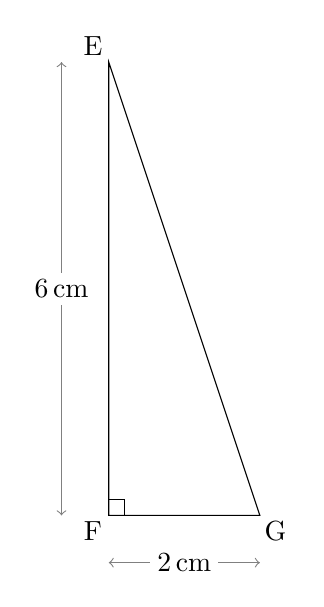
\begin{tikzpicture}[scale=1.0, baseline=(current bounding box.north)]
    \begin{scope}[rotate=270]
        % Draw

        \draw (0,0) coordinate (E) --
         ++(5.757,0) coordinate (F) --
         ++(90:1.919) coordinate (G) -- cycle;

        \pic [draw, -, angle radius=0.2cm] {right angle=G--F--E};

        % Vertex LABELS
        % Labels relative to shape geometry
        \node at ($(E)+(-0.2,-0.2)$) {E};
        \node at ($(F)+(0.2,-0.2)$) {F};
        \node at ($(G)+(0.2,0.2)$) {G};


        % dotted/dashed arrows shifted away from edges
        % Horizontal side (A-B), shifted down
        \draw[<->, gray]
            ($(E) + (0,-0.6cm)$) -- ($(F) + (0,-0.6cm)$)
            node[black, midway, fill=white, inner sep=2.5pt] {6\,cm};

        % Vertical side (B-C), shifted right
        \draw[<->, gray]
            ($(F) + (0.6cm,0)$) -- ($(G) + (0.6cm,0)$)
            node[black, midway, fill=white, xshift=0mm, inner sep=2.5pt] {2\,cm};

    \end{scope}
\end{tikzpicture}
\end{minipage}%
\hfill
\begin{minipage}{.4\textwidth}
  \begin{align*}
    \text{Area} &= \frac{1}{2} \text{bh} \\
    \text{Area} &= \frac{1}{2} \times 6 \text{cm} \times 2 \text{cm}  \\
    \text{Area} &= 6.0 \text{cm}^2
  \end{align*}
\end{minipage}

\par\vspace{1cm}\begin{minipage}{0.55\textwidth}
  \refstepcounter{minipagecount}
  \noindent{(\theminipagecount)}\quad
 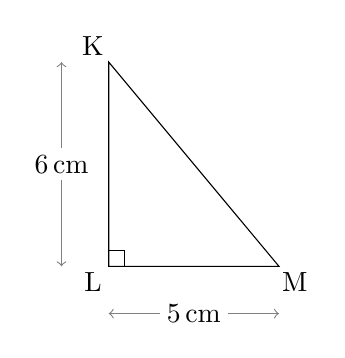
\begin{tikzpicture}[scale=1.0, baseline=(current bounding box.north)]
    \begin{scope}[rotate=270]
        % Draw

        \draw (0,0) coordinate (K) --
         ++(2.594,0) coordinate (L) --
         ++(90:2.162) coordinate (M) -- cycle;

        \pic [draw, -, angle radius=0.2cm] {right angle=M--L--K};

        % Vertex LABELS
        % Labels relative to shape geometry
        \node at ($(K)+(-0.2,-0.2)$) {K};
        \node at ($(L)+(0.2,-0.2)$) {L};
        \node at ($(M)+(0.2,0.2)$) {M};


        % dotted/dashed arrows shifted away from edges
        % Horizontal side (A-B), shifted down
        \draw[<->, gray]
            ($(K) + (0,-0.6cm)$) -- ($(L) + (0,-0.6cm)$)
            node[black, midway, fill=white, inner sep=2.5pt] {6\,cm};

        % Vertical side (B-C), shifted right
        \draw[<->, gray]
            ($(L) + (0.6cm,0)$) -- ($(M) + (0.6cm,0)$)
            node[black, midway, fill=white, xshift=0mm, inner sep=2.5pt] {5\,cm};

    \end{scope}
\end{tikzpicture}
\end{minipage}%
\hfill
\begin{minipage}{.4\textwidth}
  \begin{align*}
    \text{Area} &= \frac{1}{2} \text{bh} \\
    \text{Area} &= \frac{1}{2} \times 6 \text{cm} \times 5 \text{cm}  \\
    \text{Area} &= 15.0 \text{cm}^2
  \end{align*}
\end{minipage}

\par\vspace{1cm}\begin{minipage}{0.55\textwidth}
  \refstepcounter{minipagecount}
  \noindent{(\theminipagecount)}\quad
 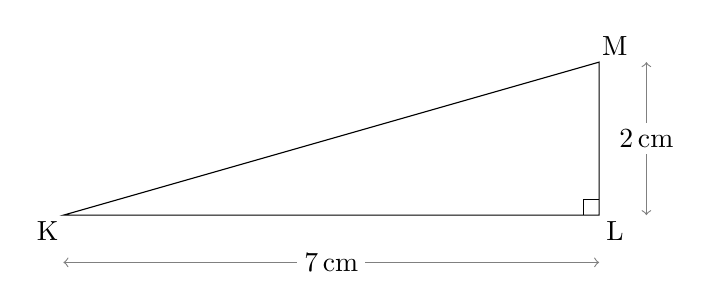
\begin{tikzpicture}[scale=1.0, baseline=(current bounding box.north)]
    \begin{scope}[rotate=0]
        % Draw

        \draw (0,0) coordinate (K) --
         ++(6.804,0) coordinate (L) --
         ++(90:1.944) coordinate (M) -- cycle;

        \pic [draw, -, angle radius=0.2cm] {right angle=M--L--K};

        % Vertex LABELS
        % Labels relative to shape geometry
        \node at ($(K)+(-0.2,-0.2)$) {K};
        \node at ($(L)+(0.2,-0.2)$) {L};
        \node at ($(M)+(0.2,0.2)$) {M};


        % dotted/dashed arrows shifted away from edges
        % Horizontal side (A-B), shifted down
        \draw[<->, gray]
            ($(K) + (0,-0.6cm)$) -- ($(L) + (0,-0.6cm)$)
            node[black, midway, fill=white, inner sep=2.5pt] {7\,cm};

        % Vertical side (B-C), shifted right
        \draw[<->, gray]
            ($(L) + (0.6cm,0)$) -- ($(M) + (0.6cm,0)$)
            node[black, midway, fill=white, xshift=0mm, inner sep=2.5pt] {2\,cm};

    \end{scope}
\end{tikzpicture}
\end{minipage}%
\hfill
\begin{minipage}{.4\textwidth}
  \begin{align*}
    \text{Area} &= \frac{1}{2} \text{bh} \\
    \text{Area} &= \frac{1}{2} \times 7 \text{cm} \times 2 \text{cm}  \\
    \text{Area} &= 7.0 \text{cm}^2
  \end{align*}
\end{minipage}

\par\vspace{1cm}\begin{minipage}{0.55\textwidth}
  \refstepcounter{minipagecount}
  \noindent{(\theminipagecount)}\quad
 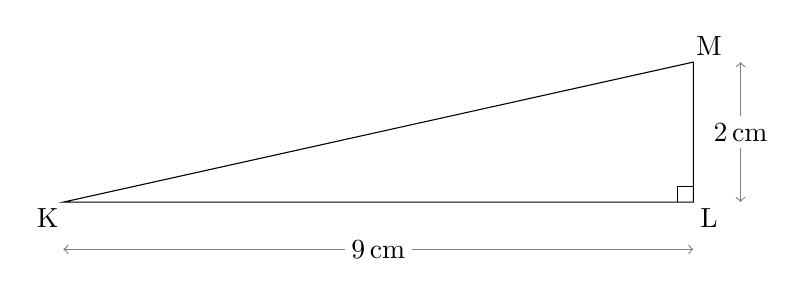
\begin{tikzpicture}[scale=1.0, baseline=(current bounding box.north)]
    \begin{scope}[rotate=0]
        % Draw

        \draw (0,0) coordinate (K) --
         ++(8.0,0) coordinate (L) --
         ++(90:1.778) coordinate (M) -- cycle;

        \pic [draw, -, angle radius=0.2cm] {right angle=M--L--K};

        % Vertex LABELS
        % Labels relative to shape geometry
        \node at ($(K)+(-0.2,-0.2)$) {K};
        \node at ($(L)+(0.2,-0.2)$) {L};
        \node at ($(M)+(0.2,0.2)$) {M};


        % dotted/dashed arrows shifted away from edges
        % Horizontal side (A-B), shifted down
        \draw[<->, gray]
            ($(K) + (0,-0.6cm)$) -- ($(L) + (0,-0.6cm)$)
            node[black, midway, fill=white, inner sep=2.5pt] {9\,cm};

        % Vertical side (B-C), shifted right
        \draw[<->, gray]
            ($(L) + (0.6cm,0)$) -- ($(M) + (0.6cm,0)$)
            node[black, midway, fill=white, xshift=0mm, inner sep=2.5pt] {2\,cm};

    \end{scope}
\end{tikzpicture}
\end{minipage}%
\hfill
\begin{minipage}{.4\textwidth}
  \begin{align*}
    \text{Area} &= \frac{1}{2} \text{bh} \\
    \text{Area} &= \frac{1}{2} \times 9 \text{cm} \times 2 \text{cm}  \\
    \text{Area} &= 9.0 \text{cm}^2
  \end{align*}
\end{minipage}

\par\vspace{1cm}\begin{minipage}{0.55\textwidth}
  \refstepcounter{minipagecount}
  \noindent{(\theminipagecount)}\quad
 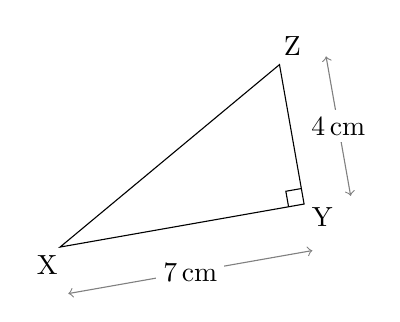
\begin{tikzpicture}[scale=1.0, baseline=(current bounding box.north)]
    \begin{scope}[rotate=10]
        % Draw

        \draw (0,0) coordinate (X) --
         ++(3.147,0) coordinate (Y) --
         ++(90:1.798) coordinate (Z) -- cycle;

        \pic [draw, -, angle radius=0.2cm] {right angle=Z--Y--X};

        % Vertex LABELS
        % Labels relative to shape geometry
        \node at ($(X)+(-0.2,-0.2)$) {X};
        \node at ($(Y)+(0.2,-0.2)$) {Y};
        \node at ($(Z)+(0.2,0.2)$) {Z};


        % dotted/dashed arrows shifted away from edges
        % Horizontal side (A-B), shifted down
        \draw[<->, gray]
            ($(X) + (0,-0.6cm)$) -- ($(Y) + (0,-0.6cm)$)
            node[black, midway, fill=white, inner sep=2.5pt] {7\,cm};

        % Vertical side (B-C), shifted right
        \draw[<->, gray]
            ($(Y) + (0.6cm,0)$) -- ($(Z) + (0.6cm,0)$)
            node[black, midway, fill=white, xshift=0mm, inner sep=2.5pt] {4\,cm};

    \end{scope}
\end{tikzpicture}
\end{minipage}%
\hfill
\begin{minipage}{.4\textwidth}
  \begin{align*}
    \text{Area} &= \frac{1}{2} \text{bh} \\
    \text{Area} &= \frac{1}{2} \times 7 \text{cm} \times 4 \text{cm}  \\
    \text{Area} &= 14.0 \text{cm}^2
  \end{align*}
\end{minipage}

\par\vspace{1cm}\begin{minipage}{0.55\textwidth}
  \refstepcounter{minipagecount}
  \noindent{(\theminipagecount)}\quad
 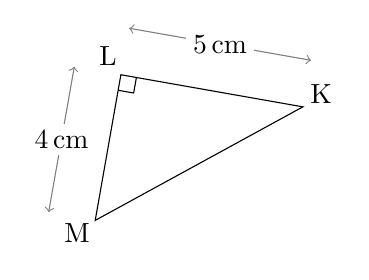
\begin{tikzpicture}[scale=1.0, baseline=(current bounding box.north)]
    \begin{scope}[rotate=170]
        % Draw

        \draw (0,0) coordinate (K) --
         ++(2.347,0) coordinate (L) --
         ++(90:1.878) coordinate (M) -- cycle;

        \pic [draw, -, angle radius=0.2cm] {right angle=M--L--K};

        % Vertex LABELS
        % Labels relative to shape geometry
        \node at ($(K)+(-0.2,-0.2)$) {K};
        \node at ($(L)+(0.2,-0.2)$) {L};
        \node at ($(M)+(0.2,0.2)$) {M};


        % dotted/dashed arrows shifted away from edges
        % Horizontal side (A-B), shifted down
        \draw[<->, gray]
            ($(K) + (0,-0.6cm)$) -- ($(L) + (0,-0.6cm)$)
            node[black, midway, fill=white, inner sep=2.5pt] {5\,cm};

        % Vertical side (B-C), shifted right
        \draw[<->, gray]
            ($(L) + (0.6cm,0)$) -- ($(M) + (0.6cm,0)$)
            node[black, midway, fill=white, xshift=0mm, inner sep=2.5pt] {4\,cm};

    \end{scope}
\end{tikzpicture}
\end{minipage}%
\hfill
\begin{minipage}{.4\textwidth}
  \begin{align*}
    \text{Area} &= \frac{1}{2} \text{bh} \\
    \text{Area} &= \frac{1}{2} \times 5 \text{cm} \times 4 \text{cm}  \\
    \text{Area} &= 10.0 \text{cm}^2
  \end{align*}
\end{minipage}

\par\vspace{1cm}\begin{minipage}{0.55\textwidth}
  \refstepcounter{minipagecount}
  \noindent{(\theminipagecount)}\quad
 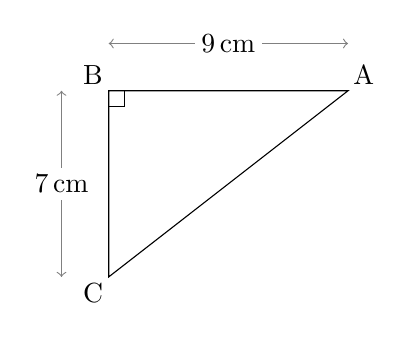
\begin{tikzpicture}[scale=1.0, baseline=(current bounding box.north)]
    \begin{scope}[rotate=180]
        % Draw

        \draw (0,0) coordinate (A) --
         ++(3.039,0) coordinate (B) --
         ++(90:2.364) coordinate (C) -- cycle;

        \pic [draw, -, angle radius=0.2cm] {right angle=C--B--A};

        % Vertex LABELS
        % Labels relative to shape geometry
        \node at ($(A)+(-0.2,-0.2)$) {A};
        \node at ($(B)+(0.2,-0.2)$) {B};
        \node at ($(C)+(0.2,0.2)$) {C};


        % dotted/dashed arrows shifted away from edges
        % Horizontal side (A-B), shifted down
        \draw[<->, gray]
            ($(A) + (0,-0.6cm)$) -- ($(B) + (0,-0.6cm)$)
            node[black, midway, fill=white, inner sep=2.5pt] {9\,cm};

        % Vertical side (B-C), shifted right
        \draw[<->, gray]
            ($(B) + (0.6cm,0)$) -- ($(C) + (0.6cm,0)$)
            node[black, midway, fill=white, xshift=0mm, inner sep=2.5pt] {7\,cm};

    \end{scope}
\end{tikzpicture}
\end{minipage}%
\hfill
\begin{minipage}{.4\textwidth}
  \begin{align*}
    \text{Area} &= \frac{1}{2} \text{bh} \\
    \text{Area} &= \frac{1}{2} \times 9 \text{cm} \times 7 \text{cm}  \\
    \text{Area} &= 31.5 \text{cm}^2
  \end{align*}
\end{minipage}

\par\vspace{1cm}\begin{minipage}{0.55\textwidth}
  \refstepcounter{minipagecount}
  \noindent{(\theminipagecount)}\quad
 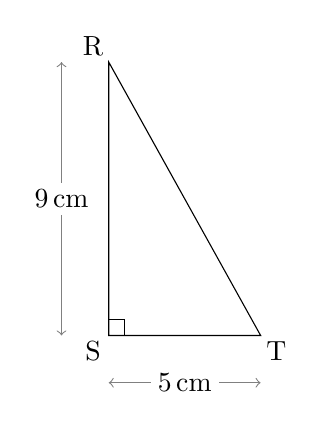
\begin{tikzpicture}[scale=1.0, baseline=(current bounding box.north)]
    \begin{scope}[rotate=270]
        % Draw

        \draw (0,0) coordinate (R) --
         ++(3.472,0) coordinate (S) --
         ++(90:1.929) coordinate (T) -- cycle;

        \pic [draw, -, angle radius=0.2cm] {right angle=T--S--R};

        % Vertex LABELS
        % Labels relative to shape geometry
        \node at ($(R)+(-0.2,-0.2)$) {R};
        \node at ($(S)+(0.2,-0.2)$) {S};
        \node at ($(T)+(0.2,0.2)$) {T};


        % dotted/dashed arrows shifted away from edges
        % Horizontal side (A-B), shifted down
        \draw[<->, gray]
            ($(R) + (0,-0.6cm)$) -- ($(S) + (0,-0.6cm)$)
            node[black, midway, fill=white, inner sep=2.5pt] {9\,cm};

        % Vertical side (B-C), shifted right
        \draw[<->, gray]
            ($(S) + (0.6cm,0)$) -- ($(T) + (0.6cm,0)$)
            node[black, midway, fill=white, xshift=0mm, inner sep=2.5pt] {5\,cm};

    \end{scope}
\end{tikzpicture}
\end{minipage}%
\hfill
\begin{minipage}{.4\textwidth}
  \begin{align*}
    \text{Area} &= \frac{1}{2} \text{bh} \\
    \text{Area} &= \frac{1}{2} \times 9 \text{cm} \times 5 \text{cm}  \\
    \text{Area} &= 22.5 \text{cm}^2
  \end{align*}
\end{minipage}

\par\vspace{1cm}\begin{minipage}{0.55\textwidth}
  \refstepcounter{minipagecount}
  \noindent{(\theminipagecount)}\quad
 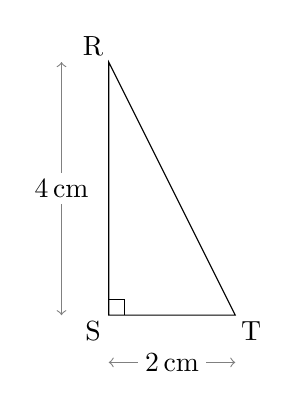
\begin{tikzpicture}[scale=1.0, baseline=(current bounding box.north)]
    \begin{scope}[rotate=270]
        % Draw

        \draw (0,0) coordinate (R) --
         ++(3.214,0) coordinate (S) --
         ++(90:1.607) coordinate (T) -- cycle;

        \pic [draw, -, angle radius=0.2cm] {right angle=T--S--R};

        % Vertex LABELS
        % Labels relative to shape geometry
        \node at ($(R)+(-0.2,-0.2)$) {R};
        \node at ($(S)+(0.2,-0.2)$) {S};
        \node at ($(T)+(0.2,0.2)$) {T};


        % dotted/dashed arrows shifted away from edges
        % Horizontal side (A-B), shifted down
        \draw[<->, gray]
            ($(R) + (0,-0.6cm)$) -- ($(S) + (0,-0.6cm)$)
            node[black, midway, fill=white, inner sep=2.5pt] {4\,cm};

        % Vertical side (B-C), shifted right
        \draw[<->, gray]
            ($(S) + (0.6cm,0)$) -- ($(T) + (0.6cm,0)$)
            node[black, midway, fill=white, xshift=0mm, inner sep=2.5pt] {2\,cm};

    \end{scope}
\end{tikzpicture}
\end{minipage}%
\hfill
\begin{minipage}{.4\textwidth}
  \begin{align*}
    \text{Area} &= \frac{1}{2} \text{bh} \\
    \text{Area} &= \frac{1}{2} \times 4 \text{cm} \times 2 \text{cm}  \\
    \text{Area} &= 4.0 \text{cm}^2
  \end{align*}
\end{minipage}

\par\vspace{1cm}\begin{minipage}{0.55\textwidth}
  \refstepcounter{minipagecount}
  \noindent{(\theminipagecount)}\quad
 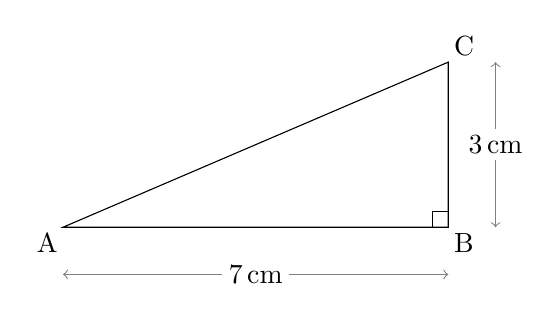
\begin{tikzpicture}[scale=1.0, baseline=(current bounding box.north)]
    \begin{scope}[rotate=0]
        % Draw

        \draw (0,0) coordinate (A) --
         ++(4.893,0) coordinate (B) --
         ++(90:2.097) coordinate (C) -- cycle;

        \pic [draw, -, angle radius=0.2cm] {right angle=C--B--A};

        % Vertex LABELS
        % Labels relative to shape geometry
        \node at ($(A)+(-0.2,-0.2)$) {A};
        \node at ($(B)+(0.2,-0.2)$) {B};
        \node at ($(C)+(0.2,0.2)$) {C};


        % dotted/dashed arrows shifted away from edges
        % Horizontal side (A-B), shifted down
        \draw[<->, gray]
            ($(A) + (0,-0.6cm)$) -- ($(B) + (0,-0.6cm)$)
            node[black, midway, fill=white, inner sep=2.5pt] {7\,cm};

        % Vertical side (B-C), shifted right
        \draw[<->, gray]
            ($(B) + (0.6cm,0)$) -- ($(C) + (0.6cm,0)$)
            node[black, midway, fill=white, xshift=0mm, inner sep=2.5pt] {3\,cm};

    \end{scope}
\end{tikzpicture}
\end{minipage}%
\hfill
\begin{minipage}{.4\textwidth}
  \begin{align*}
    \text{Area} &= \frac{1}{2} \text{bh} \\
    \text{Area} &= \frac{1}{2} \times 7 \text{cm} \times 3 \text{cm}  \\
    \text{Area} &= 10.5 \text{cm}^2
  \end{align*}
\end{minipage}

\par\vspace{1cm}\begin{minipage}{0.55\textwidth}
  \refstepcounter{minipagecount}
  \noindent{(\theminipagecount)}\quad
 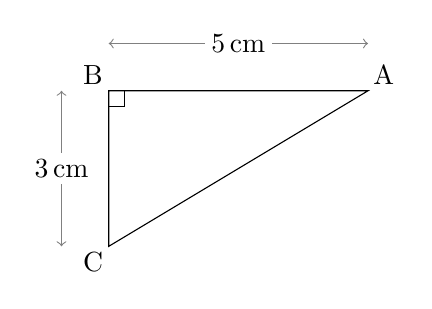
\begin{tikzpicture}[scale=1.0, baseline=(current bounding box.north)]
    \begin{scope}[rotate=180]
        % Draw

        \draw (0,0) coordinate (A) --
         ++(3.293,0) coordinate (B) --
         ++(90:1.976) coordinate (C) -- cycle;

        \pic [draw, -, angle radius=0.2cm] {right angle=C--B--A};

        % Vertex LABELS
        % Labels relative to shape geometry
        \node at ($(A)+(-0.2,-0.2)$) {A};
        \node at ($(B)+(0.2,-0.2)$) {B};
        \node at ($(C)+(0.2,0.2)$) {C};


        % dotted/dashed arrows shifted away from edges
        % Horizontal side (A-B), shifted down
        \draw[<->, gray]
            ($(A) + (0,-0.6cm)$) -- ($(B) + (0,-0.6cm)$)
            node[black, midway, fill=white, inner sep=2.5pt] {5\,cm};

        % Vertical side (B-C), shifted right
        \draw[<->, gray]
            ($(B) + (0.6cm,0)$) -- ($(C) + (0.6cm,0)$)
            node[black, midway, fill=white, xshift=0mm, inner sep=2.5pt] {3\,cm};

    \end{scope}
\end{tikzpicture}
\end{minipage}%
\hfill
\begin{minipage}{.4\textwidth}
  \begin{align*}
    \text{Area} &= \frac{1}{2} \text{bh} \\
    \text{Area} &= \frac{1}{2} \times 5 \text{cm} \times 3 \text{cm}  \\
    \text{Area} &= 7.5 \text{cm}^2
  \end{align*}
\end{minipage}

\par\vspace{1cm}\begin{minipage}{0.55\textwidth}
  \refstepcounter{minipagecount}
  \noindent{(\theminipagecount)}\quad
 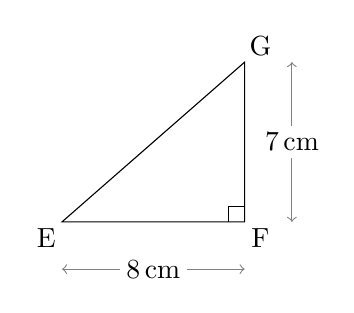
\begin{tikzpicture}[scale=1.0, baseline=(current bounding box.north)]
    \begin{scope}[rotate=0]
        % Draw

        \draw (0,0) coordinate (E) --
         ++(2.319,0) coordinate (F) --
         ++(90:2.029) coordinate (G) -- cycle;

        \pic [draw, -, angle radius=0.2cm] {right angle=G--F--E};

        % Vertex LABELS
        % Labels relative to shape geometry
        \node at ($(E)+(-0.2,-0.2)$) {E};
        \node at ($(F)+(0.2,-0.2)$) {F};
        \node at ($(G)+(0.2,0.2)$) {G};


        % dotted/dashed arrows shifted away from edges
        % Horizontal side (A-B), shifted down
        \draw[<->, gray]
            ($(E) + (0,-0.6cm)$) -- ($(F) + (0,-0.6cm)$)
            node[black, midway, fill=white, inner sep=2.5pt] {8\,cm};

        % Vertical side (B-C), shifted right
        \draw[<->, gray]
            ($(F) + (0.6cm,0)$) -- ($(G) + (0.6cm,0)$)
            node[black, midway, fill=white, xshift=0mm, inner sep=2.5pt] {7\,cm};

    \end{scope}
\end{tikzpicture}
\end{minipage}%
\hfill
\begin{minipage}{.4\textwidth}
  \begin{align*}
    \text{Area} &= \frac{1}{2} \text{bh} \\
    \text{Area} &= \frac{1}{2} \times 8 \text{cm} \times 7 \text{cm}  \\
    \text{Area} &= 28.0 \text{cm}^2
  \end{align*}
\end{minipage}

\par\vspace{1cm}\begin{minipage}{0.55\textwidth}
  \refstepcounter{minipagecount}
  \noindent{(\theminipagecount)}\quad
 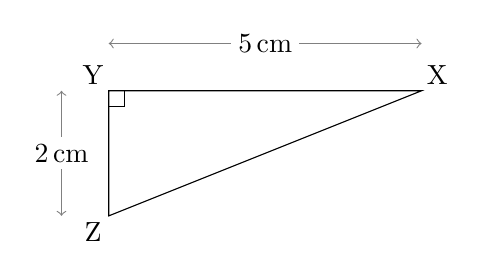
\begin{tikzpicture}[scale=1.0, baseline=(current bounding box.north)]
    \begin{scope}[rotate=180]
        % Draw

        \draw (0,0) coordinate (X) --
         ++(3.973,0) coordinate (Y) --
         ++(90:1.589) coordinate (Z) -- cycle;

        \pic [draw, -, angle radius=0.2cm] {right angle=Z--Y--X};

        % Vertex LABELS
        % Labels relative to shape geometry
        \node at ($(X)+(-0.2,-0.2)$) {X};
        \node at ($(Y)+(0.2,-0.2)$) {Y};
        \node at ($(Z)+(0.2,0.2)$) {Z};


        % dotted/dashed arrows shifted away from edges
        % Horizontal side (A-B), shifted down
        \draw[<->, gray]
            ($(X) + (0,-0.6cm)$) -- ($(Y) + (0,-0.6cm)$)
            node[black, midway, fill=white, inner sep=2.5pt] {5\,cm};

        % Vertical side (B-C), shifted right
        \draw[<->, gray]
            ($(Y) + (0.6cm,0)$) -- ($(Z) + (0.6cm,0)$)
            node[black, midway, fill=white, xshift=0mm, inner sep=2.5pt] {2\,cm};

    \end{scope}
\end{tikzpicture}
\end{minipage}%
\hfill
\begin{minipage}{.4\textwidth}
  \begin{align*}
    \text{Area} &= \frac{1}{2} \text{bh} \\
    \text{Area} &= \frac{1}{2} \times 5 \text{cm} \times 2 \text{cm}  \\
    \text{Area} &= 5.0 \text{cm}^2
  \end{align*}
\end{minipage}

\par\vspace{1cm}\begin{minipage}{0.55\textwidth}
  \refstepcounter{minipagecount}
  \noindent{(\theminipagecount)}\quad
 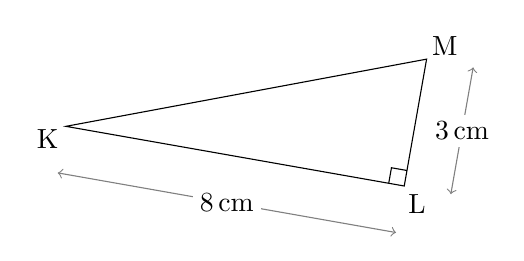
\begin{tikzpicture}[scale=1.0, baseline=(current bounding box.north)]
    \begin{scope}[rotate=-10]
        % Draw

        \draw (0,0) coordinate (K) --
         ++(4.363,0) coordinate (L) --
         ++(90:1.636) coordinate (M) -- cycle;

        \pic [draw, -, angle radius=0.2cm] {right angle=M--L--K};

        % Vertex LABELS
        % Labels relative to shape geometry
        \node at ($(K)+(-0.2,-0.2)$) {K};
        \node at ($(L)+(0.2,-0.2)$) {L};
        \node at ($(M)+(0.2,0.2)$) {M};


        % dotted/dashed arrows shifted away from edges
        % Horizontal side (A-B), shifted down
        \draw[<->, gray]
            ($(K) + (0,-0.6cm)$) -- ($(L) + (0,-0.6cm)$)
            node[black, midway, fill=white, inner sep=2.5pt] {8\,cm};

        % Vertical side (B-C), shifted right
        \draw[<->, gray]
            ($(L) + (0.6cm,0)$) -- ($(M) + (0.6cm,0)$)
            node[black, midway, fill=white, xshift=0mm, inner sep=2.5pt] {3\,cm};

    \end{scope}
\end{tikzpicture}
\end{minipage}%
\hfill
\begin{minipage}{.4\textwidth}
  \begin{align*}
    \text{Area} &= \frac{1}{2} \text{bh} \\
    \text{Area} &= \frac{1}{2} \times 8 \text{cm} \times 3 \text{cm}  \\
    \text{Area} &= 12.0 \text{cm}^2
  \end{align*}
\end{minipage}

\par\vspace{1cm}\begin{minipage}{0.55\textwidth}
  \refstepcounter{minipagecount}
  \noindent{(\theminipagecount)}\quad
 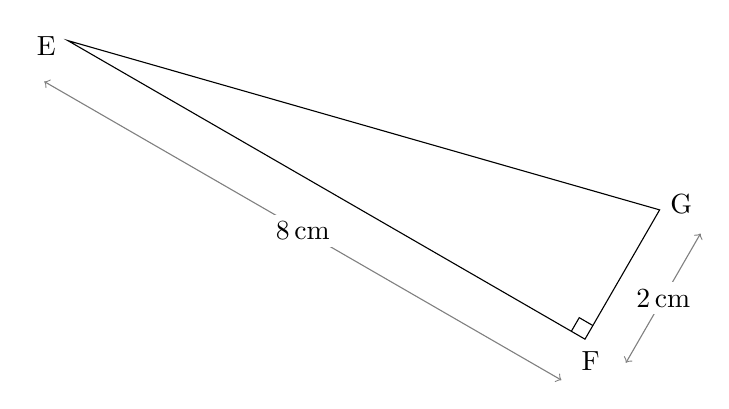
\begin{tikzpicture}[scale=1.0, baseline=(current bounding box.north)]
    \begin{scope}[rotate=-30]
        % Draw

        \draw (0,0) coordinate (E) --
         ++(7.584,0) coordinate (F) --
         ++(90:1.896) coordinate (G) -- cycle;

        \pic [draw, -, angle radius=0.2cm] {right angle=G--F--E};

        % Vertex LABELS
        % Labels relative to shape geometry
        \node at ($(E)+(-0.2,-0.2)$) {E};
        \node at ($(F)+(0.2,-0.2)$) {F};
        \node at ($(G)+(0.2,0.2)$) {G};


        % dotted/dashed arrows shifted away from edges
        % Horizontal side (A-B), shifted down
        \draw[<->, gray]
            ($(E) + (0,-0.6cm)$) -- ($(F) + (0,-0.6cm)$)
            node[black, midway, fill=white, inner sep=2.5pt] {8\,cm};

        % Vertical side (B-C), shifted right
        \draw[<->, gray]
            ($(F) + (0.6cm,0)$) -- ($(G) + (0.6cm,0)$)
            node[black, midway, fill=white, xshift=0mm, inner sep=2.5pt] {2\,cm};

    \end{scope}
\end{tikzpicture}
\end{minipage}%
\hfill
\begin{minipage}{.4\textwidth}
  \begin{align*}
    \text{Area} &= \frac{1}{2} \text{bh} \\
    \text{Area} &= \frac{1}{2} \times 8 \text{cm} \times 2 \text{cm}  \\
    \text{Area} &= 8.0 \text{cm}^2
  \end{align*}
\end{minipage}

\par\vspace{1cm}\begin{minipage}{0.55\textwidth}
  \refstepcounter{minipagecount}
  \noindent{(\theminipagecount)}\quad
 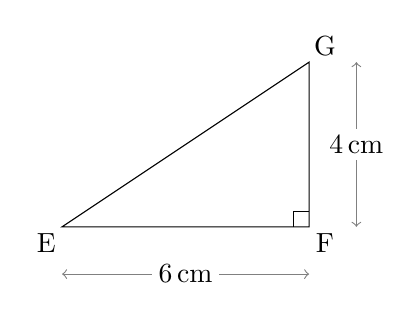
\begin{tikzpicture}[scale=1.0, baseline=(current bounding box.north)]
    \begin{scope}[rotate=0]
        % Draw

        \draw (0,0) coordinate (E) --
         ++(3.138,0) coordinate (F) --
         ++(90:2.092) coordinate (G) -- cycle;

        \pic [draw, -, angle radius=0.2cm] {right angle=G--F--E};

        % Vertex LABELS
        % Labels relative to shape geometry
        \node at ($(E)+(-0.2,-0.2)$) {E};
        \node at ($(F)+(0.2,-0.2)$) {F};
        \node at ($(G)+(0.2,0.2)$) {G};


        % dotted/dashed arrows shifted away from edges
        % Horizontal side (A-B), shifted down
        \draw[<->, gray]
            ($(E) + (0,-0.6cm)$) -- ($(F) + (0,-0.6cm)$)
            node[black, midway, fill=white, inner sep=2.5pt] {6\,cm};

        % Vertical side (B-C), shifted right
        \draw[<->, gray]
            ($(F) + (0.6cm,0)$) -- ($(G) + (0.6cm,0)$)
            node[black, midway, fill=white, xshift=0mm, inner sep=2.5pt] {4\,cm};

    \end{scope}
\end{tikzpicture}
\end{minipage}%
\hfill
\begin{minipage}{.4\textwidth}
  \begin{align*}
    \text{Area} &= \frac{1}{2} \text{bh} \\
    \text{Area} &= \frac{1}{2} \times 6 \text{cm} \times 4 \text{cm}  \\
    \text{Area} &= 12.0 \text{cm}^2
  \end{align*}
\end{minipage}

\par\vspace{1cm}\begin{minipage}{0.55\textwidth}
  \refstepcounter{minipagecount}
  \noindent{(\theminipagecount)}\quad
 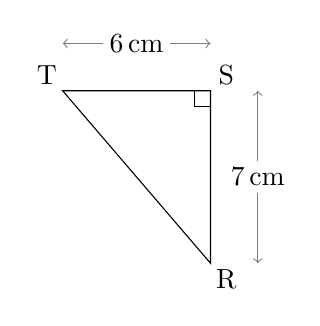
\begin{tikzpicture}[scale=1.0, baseline=(current bounding box.north)]
    \begin{scope}[rotate=90]
        % Draw

        \draw (0,0) coordinate (R) --
         ++(2.191,0) coordinate (S) --
         ++(90:1.878) coordinate (T) -- cycle;

        \pic [draw, -, angle radius=0.2cm] {right angle=T--S--R};

        % Vertex LABELS
        % Labels relative to shape geometry
        \node at ($(R)+(-0.2,-0.2)$) {R};
        \node at ($(S)+(0.2,-0.2)$) {S};
        \node at ($(T)+(0.2,0.2)$) {T};


        % dotted/dashed arrows shifted away from edges
        % Horizontal side (A-B), shifted down
        \draw[<->, gray]
            ($(R) + (0,-0.6cm)$) -- ($(S) + (0,-0.6cm)$)
            node[black, midway, fill=white, inner sep=2.5pt] {7\,cm};

        % Vertical side (B-C), shifted right
        \draw[<->, gray]
            ($(S) + (0.6cm,0)$) -- ($(T) + (0.6cm,0)$)
            node[black, midway, fill=white, xshift=0mm, inner sep=2.5pt] {6\,cm};

    \end{scope}
\end{tikzpicture}
\end{minipage}%
\hfill
\begin{minipage}{.4\textwidth}
  \begin{align*}
    \text{Area} &= \frac{1}{2} \text{bh} \\
    \text{Area} &= \frac{1}{2} \times 7 \text{cm} \times 6 \text{cm}  \\
    \text{Area} &= 21.0 \text{cm}^2
  \end{align*}
\end{minipage}

\par\vspace{1cm}

\end{document}
